     %%%%%%%%%%%%%%%%%%%%
     %                  %
     %  capitolo3.tex   %
     %                  %
     %%%%%%%%%%%%%%%%%%%%
     
\chapter{The $O(N)$ model at $O(\partial^2)$ of the derivative expansion}
\noindent
In this chapter I will apply the concepts illustrated in the previous one to a concrete model, the $O(N)$ model, 
which describes the behavior of an $N$-components real scalar field $\phi^a(x)$ with an $O(N)$ rotational invariance in vector representation. 


Due to its simplicity and to the wide number of physical systems it's able to describe, the $O(N)$ model is one of the most studied in 
modern theoretical physics. 
As an example, I remember here just some of the systems described using that as theoretical framework:
\begin{enumerate}
 \item polymers, for $N = 0$ \cite{polimeri};
 \item the Ising model, for $N = 1$ \cite{ising};
 \item the XY model, for $N = 2$ \cite{xy};
 \item the Heisemberg model, for $N = 3$ \cite{Polyakov};
 \item chiral effective model for QCD, for $N = 4$\cite{hidaka};
 \item theory of high $T_c$ sperconductivity, for $N = 5$\cite{super};
\end{enumerate}
Moreover, also the Higgs field of the Standard Model is based on a linear complex $O(N)$ model.

The approximation scheme I'll use on the \emph{effective average action} in order to solve the Wetterich equation
\eqref{wetterich} is a derivative expansion up to order $O(\partial^2)$ (naturally the derivative expansion is consistent with the $O(N)$ symmetry).
So we have the following expression for $\Gamma_k$:
\begin{equation}\label{azioneefficace}
 \Gamma_k (\phi) = \int d^Dx \left[  U_k(\rho) + \frac{Z_k(\rho)}{2} \partial^\mu \phi_a(x) \partial_\mu \phi^a(x) + \frac{Y_k(\rho)}{4} \partial^\mu \rho(x) \partial_\mu \rho(x) + \mathcal{O}(\partial^4)\right]
\end{equation}
where I have defined $\rho(x) = \frac{1}{2}\phi^a(x)\phi_a(x)$.
The effective potential $U_k(\rho)$ is the observable that permit us to study the ground state of a given theory as well as the basics interactions, while the kinetic term involve two different renormalization functions, $Z_k(\rho)$ and $Y_k(\rho)$.
For $N > 1$ the first one, $Z_k(\rho)$, is related to the renormalization of the Goldstone modes, whereas the renormalization of the radial mode involves both $Z_k(\rho)$ and $Y_k(\rho)$.
To maximally simplify our model we will allow $U_k(\rho)$, $Z_k(\rho)$ and $Y_k(\rho)$ to depends just on $\rho$ and not explicitly on the spacetime position.
In this framework, the evolution equation for $\Gamma_k$ reduces to a system of coupled nonlinear differential equations for the three functions $U_k(\rho)$, $Z_k(\rho)$ and $Y_k(\rho)$.
These evolution equations will be derived in the following, also considering the special case $N\to \infty$,
to eventually study scaling solutions (fixed point configurations of the function space). 


\section{Exact evolution equation for the effective potential}
In order to obtain the FRG flow equation for the effective potential, I will set constant field couplings in the Hessian $\Gamma^{(2)}$.

So, the effective average action is:
\begin{equation}
\Gamma_k(\phi) \approx \int U_k{(\rho)} d^Dx = V_D U_k{(\rho)}
\end{equation}
Where $V_D\equiv\int d^D x$ is the volume in the  $D-$dimensional euclidean space where the physical system under consideration is confined. Now we can trivially obtain the effective potential flow equation:
\begin{equation}\label{esempiosopra}
 \dot{U}_k{(\rho)} = \frac{1}{2V_D} \Tr\left\{ \frac{\dot{R}_k}{{\Gamma_k}^{(2)} + R_k}\right\}
\end{equation}
In momentum space:
\begin{equation}\label{...}
\dot{U}_k(\rho) = \frac{1}{2V_D}\sum_{ab} \int d^Dx \int d^D y \int \frac{d^Dp}{(2\pi)^D} \int \frac{d^Dq}{(2\pi)^D} {G}^{a}_a(p^2)\dot{R}_k(q^2) e ^{i(x-y)(p-q)}
\end{equation}
In order to avoid excessive formalism, I will use the same notation for functions or operators in coordinate space and for their Fourier transform.
So, for example the momentum space expression for the exact propagator and the dotted regulator function appearing in \eqref{esempiosopra} read:
\begin{displaymath}
\left.
\begin{array}{l}
 {G_k}^{ab} (x-y) = \int \frac{d^Dp}{(2\pi)^D} {G}^{ab}(p) e^{i(x-y)p}  \\
  \\
 {\dot{R}_k}^{ba} (y-x) =  \delta^{ba} \int \frac{d^Dq}{(2\pi)^D} \dot{R}_k(q^2) e ^{i(y-x)q}\\

 \end{array} 
\right.
\end{displaymath}
I also remark that, because our model involve real scalar fields in coordinate space, in momentum space we have:
$$\phi_a(q) = \phi^*_a(-q)$$
because of the definition of Fourier transorm: 
$$ \phi_a(q) = \int \phi(x) \e^{iqx}d^Dx$$
In the integral in \eqref{...} I'll introduce the variable $ z = y - x $ and, after performing the $z$ and the $x$ integrals, the result is:
\begin{equation}\label{settte}
\dot{U}_k(\rho) = \sum_{a} \int \frac{d^Dq}{(2\pi)^D} {G}^{a}_{k\ a}(q^2)R_k(q^2)
\end{equation}
To perform the integration in $q$ we will use the polar coordinate system in a $D-$dimensional space:
\begin{equation}
 \int \frac{d^Dq}{(2\pi)^D} = 4v_D \int_0^\infty q^{D-1}dq
\end{equation}
I have already performed the integral over the $D$-dimensional solid angle, because of the angular independence of the integrand \eqref{settte} and
I have also defined, for the sake of brevity, the numerical factor $v_D$:
$$v_D = \frac{1}{2^{D+1}\Gamma(\frac{D}{2})(\pi)^\frac{D}{2}}$$
So the  \eqref{settte} becomes:
\begin{equation}
\dot{U}(\rho) = \sum_{a} 2v_D \int_0^\infty q^{D-1}  {G}^{a}_{k\ a}(q)\dot{R}_k(q^2)dq
\end{equation}
The trace of the exact propagator is:
\begin{equation*}\label{uuu}
 {G}^a_a(q^2) = \Big[\Gamma^{(2)}_k(q^2) + R_k(q^2)\Big]^{-1} = 
\end{equation*}
$$\frac{\delta^a_{a} - \widehat{\phi}^{a}\widehat{\phi}_{a}}{U'_k(\rho) +  Z_k({\rho})q^2 + R_k(q^2) }  + \frac{\widehat{\phi}^{a}\widehat{\phi}_{a}}{ U'(\rho) +  2\bar{\rho}U''_k(\rho)+ [Z_k(\bar{\rho}) + {\rho}Y_k(\bar{\rho})]q^2 + R_k(q^2)} =$$
\begin{equation}\label{vvvvvv}
 \frac{N-1}{U'_k(\rho) +  Z_k({\rho})q^2 + R_k(q^2)}  + \frac{1}{U'(\rho) +  2{\rho}U''_k(\rho)+ [Z_k({\rho}) + {\rho}Y_k({\rho})]q^2 + R_k(q^2)} 
\end{equation}
where I have defined:
\begin{equation}
\widehat{\phi}_{a} = \frac{\bar{\phi}_{a}}{\sqrt{2\bar{\rho}}}
\end{equation}
So $\delta^{ab} - \widehat{\phi}^{a}\widehat{\phi}^{b}$ and $\widehat{\phi}^{a}\widehat{\phi}^{b}$ are the projectors on the longitudinal and on the transverse directions respectively.

We can substitute equation \eqref{vvvvvv} in  \eqref{uuu}, obtaining:
\begin{equation}\label{upunto}
\dot{U}(\rho) =   2v_D  \int_0^\infty q^{D-1}  \dot{R}_k(q^2) \left[  {(N-1)}{G_\perp(q^2)}  + {G_\parallel(q^2)}\right] dq
\end{equation}
Where I have defined, for the sake of simplicity the transverse component of the propagator and the longitudinal one, in the following way:
$$G_\perp (q)= \frac{1}{U'_k(\rho) +  Z_k({\rho})q^2 + R_k(q) } $$
$$G_\parallel (q) = \frac{1}{U'(\rho) + 2\bar{\rho}U''_k(\rho) +  (Z_k({\rho}) + \bar{\rho}Y_k(\bar{\rho}))q^2 + R_k(q)}$$
So the propagator can be written in the following way:
\begin{equation}
 G^{ab}(q) = (\delta^{ab} - \widehat{\phi}^a\widehat{\phi}^b)G_\perp (q) + \widehat{\phi}^a\widehat{\phi}^bG_\parallel (q)
\end{equation}
For $\rho \neq 0$ it's easy to identify the first term as the contribution from the $N-1$ Goldstone bosons and the first one as the contribution from the radial mode.
The exact evolution equation for the effective potential can be interpreted in a graphical way in terms of a $1$-loop Feynman-like diagrams, as shown in Fig.\ref{fig:looppot}.
\begin{figure}
\begin{center}
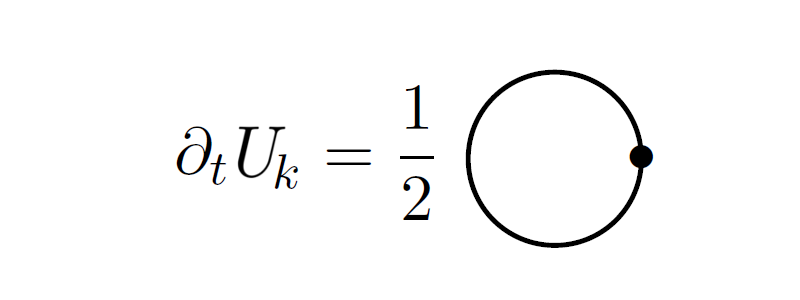
\includegraphics[scale=0.4]{Immagini/potenziale.png}
\caption{A Feynman-like graph representation for the exact evolution equation for the effective potential $U_k(\rho)$.}
\label{fig:looppot}
\end{center}
\end{figure}

In order to study the behavior of the effective potential, an approximation that is widely used in the literature is the LPA (Local Potential Approximation).
The LPA result consists in setting $Z=1$ and $Y=0$.

Although it may seems a crude approximation, the LPA is widely used in many studies, because it qualitatively reproduces most of the properties of the complete functional renormalization group description of the $O(N)$ 
model in the large distance regime, like the stability properties and number of fixed points.


\section{The equations for $\dot{Z}_k(\rho)$ and $\dot{Y}_k(\rho)$}
To go beyond the simple LPA approximation, we need to add the exact evolution equations for the non trivial $Z_k(\rho)$ and $Y_k(\rho)$. 
To derive these equations we need to know the exact evolution equation for the second order functional derivative of the effective average action,
then setting $\rho$ to a constant is sufficient to extract the flow equations.
That is what will be calculated in the following section.

\subsection{Evolution of $\Gamma_k^{(2)}$}
The procedure is very similar to what we've seen for the scalar model in the previous chapter.

The starting point is the \emph{Wetterich equation} \eqref{wetterich}. If we derive it twice with respect to the fields we obtain:
\begin{equation}\label{gamma2dot}
\dot{\Gamma}^{(2)ab}_k(x,y)= \frac{1}{2}\frac{\delta^2 }{\delta\phi_a(x)\delta\phi_b(y)}\Tr\left\{\dot{R_k}G_k\right\} 
\end{equation}
Assuming the field-independence of the functional, our problem is to calculate
the second functional derivative of the exact propagator:
$$G_k = \frac{1}{{\Gamma_k}^{(2)} + R_k}$$
We apply the well-known formula for the derivative of a matrix, knowing the expression of its inverse:
$$\frac{\partial^2}{\partial x\partial y} M^{-1} = $$
$$M^{-1}\left(\frac{\partial}{\partial x} M \right)M^{-1}\left(\frac{\partial}{\partial y} M \right) M^{-1} + M^{-1}\left(\frac{\partial}{\partial y} M \right)M^{-1}\left(\frac{\partial}{\partial x} M \right) M^{-1} -  M^{-1}\left(\frac{\partial^2}{\partial x\partial y} M \right) M^{-1}$$
So the second functional derivative of the exact propagator is:
\begin{equation}\label{trecento11}
 \frac{\delta^2 {G^{x_1 x_2}_{a_1a_2}}_k }{\delta \phi_a(x) \delta \phi_b(y)}= {G^{x_1 x_3}_{a_1a_3}}_k \left[ 2\frac{\delta {\Gamma^{(2)x_3 x_4}_{a_3a_4}}}{\delta \phi_a(x)}{G_{a_4a_5}^{x_4x_5}}_k \frac{\delta {\Gamma_{a_5a_6}^{(2)x_5 x_6}}_k}{\delta \phi_b(y)} - \frac{\delta^2{\Gamma_{a_3a_6}^{(2)x_3x_6}}_k}{\delta \phi_a(x) \delta \phi_b(y)}\right] {G^{x_6x_2}_{a_6a_2}}_k
\end{equation}
So the trace in \eqref{gamma2dot} becomes:
\begin{equation}
\frac{1}{2}\Tr\left\{ \dot{R_k}\frac{\delta^2 }{\delta\phi_a\delta\phi_b}\frac{1}{{\Gamma_k}^{(2)} + R_k}\right\} = 
\end{equation}
\begin{equation}
 = \left[ {G^{x_1 x_3}_{a_1a_3}}_k \left(\frac{\delta {\Gamma^{(2)x_3 x_4}_{a_3a_4}}_k}{\delta \phi_a(x)}{G_{a_4a_5}^{x_4x_5}}_k \frac{\delta {\Gamma_{a_5a_6}^{(2)x_5 x_6}}_k}{\delta \phi_b(y)} - \frac{1}{2}\frac{\delta^2{\Gamma_{a_3a_6}^{(2)x_3x_6}}_k}{\delta \phi_a(x) \delta \phi_b(y)}\right) {G^{x_6x_2}_{a_6a_2}}_k \right]{\dot{R_k}_{a_2a_1}^{x_2 x_1}}\equiv A - \frac{1}{2}B
\end{equation}
Note that the evolution equations for $\Gamma^{(2)}$ involves $\Gamma^{(3)}$ and $\Gamma^{(4)}$. That's a general results, it's possible to demonstrate that the flow equation 
for $\Gamma^{(n)}$ always involves $\Gamma^{(n+1)}$ and $\Gamma^{(n+2)}$.

I'll solve the two integrals $A$ and $B$ separately in the following subsections.

\subsection*{$A$ evaluation}
If we rewrite the generalized sums explicitly in terms of spacetime integrals the expression of $A$  is 
\small{
\begin{equation}\label{quella}
\sum_{a_m}\int \left(\prod_{j=1}^6 dx_j\right) G^{a_1a_3}_k(x_3 - x_1) \frac{\delta {\Gamma^{(2)}_{a_3a_4}}_k(x_3, x_4)}{\delta \phi_a(x)}{G^{a_4a_5}_k(x_5 - x_4)} \frac{\delta {\Gamma^{a_5a_6(2)}(x_5, x_6)}_k}{\delta \phi_b(y)} G^{a_6a_2}_k(x_2 - x_6)\dot{R_k}^{a_2a_1}(x_1 - x_2)
\end{equation}}
First, I'll solve the spacetime integral. It's more convenient to work in momentum space.
The expression for the observable in \eqref{quella}   become:
\begin{displaymath}
\left.
\begin{array}{l}
G_k^{a_1a_3} (x_3-x_1) = \int \frac{d^Dq_1}{(2\pi)^D}  {G}_k^{a_1a_3}(q_1) e^{i(x_3-x_1)q_1}\\ \\
G_k^{a_4a_5} (x_5-x_4) = \int \frac{d^Dq_2}{(2\pi)^D}  {G}_k^{a_4a_5}(q_2) e^{i(x_5-x_4)q_2}\\ \\
G_k^{a_6a_2} (x_2-x_6) = \int \frac{d^Dq_3}{(2\pi)^D}  {G}_k^{a_6a_2}(q_3) e^{i(x_2-x_6)q_3}\\ \\
\Gamma^{(3)aa_3a_4} (x, x_3, x_4) = \int \frac{d^Dp_1}{(2\pi)^D}\int \frac{d^Dp_2}{(2\pi)^D}\int \frac{d^Dp_3}{(2\pi)^D} {\Gamma}^{(3)a_xa_3a_4} \delta (p_1 + p_2 + p_3) e^{ip_1x}e^{ip_2x_3}e^{ip_3x_4}\\ \\	
\Gamma^{(3)ba_5a_6} (y, x_5, x_6) = \int \frac{d^Dp'_1}{(2\pi)^D}\int \frac{d^Dp'_2}{(2\pi)^D}\int \frac{d^Dp'_3}{(2\pi)^D} {\Gamma}^{(3)a_ya_5a_6} \delta (p'_1 + p'_2 + p'_3) e^{ip'_1y}e^{ip'_2x_5}e^{ip'_3x_6}\\ \\
 \dot{R_k}^{a_2a_1} (x_1 - x_2) = \dot{R}_k \delta^{a_1a_2}\\ \\
\end{array}
\right.
\end{displaymath}
Substituting these expressions in \eqref{quella} and performing the spacetime integration we find the
following constraints on the moments:
\begin{center}
\begin{tabular}{cc}
$q_1 = q$ & $p_1 = p_1$\\
$q_3 = q$ & $p_1' + p_1 + q$\\
$p_2 = q$ & $p_2 = q$\\
$q_2 = -p_3$ & $p'_2 = -q$\\
$p_1' = q_2$ & $p_3 = -p_1 - q$\\
$p_2' = -q$ & $p_3' = -p_1$
\end{tabular}
\end{center}
So we can rewrite $A$ in terms of just two momenta, for example $p_1$ and $q$:
\small{
\begin{equation}\label{ja}
 A(x-y) = \sum_{a_m}\int \frac{d^Dq}{(2\pi)^D}\int \frac{d^Dp_1}{(2\pi)^D} {G}_k^{a_1a_3}(q) {\Gamma}^{(3)aa_3a_4}_{(p, q, -p-q)} {G}_k^{a_4a_5}(p_1 + q){\Gamma}^{(3)ba_5a_6}_{(-p,-q,p+q)}{G}_k^{a_6a_2}(q)\dot{R}^{a_2a_1}_k(q) e^{i(x-y)p_1}
\end{equation}}
Now, in order to obtain the momentum-space expresion for $A$ I'll perform a Fourier transform of \eqref{ja}. The result, after performing spacetime integrations in $x$ and $y$, is:
\begin{equation}
 {A}(p)=  \frac{V}{(2\pi)^D}\sum_{a_m} \int \frac{d^Dq}{(2\pi)^D} {G}_k^{a_1a_3}(q) {\Gamma}^{(3)aa_3a_4}_{(p, q, -p-q)} {G}_k^{a_4a_5}(p + q){\Gamma}^{(3)ba_5a_6}_{(-p,-q,p+q)}{G}_k^{a_6a_2}(q)\dot{R}^{a_2a_1}_k(q)
\end{equation}





\subsection*{$B$ evaluation}
The evaluation of $B$ can be performed in the same way.  In coordinate space it is:
\begin{equation}
B(x,y) = \int G^{a_1a_3}_k(x_1,x_3)\frac{\delta^2{\Gamma_{a_3a_6}^{(2)}}_k(x_3,x_6)}{\delta \phi_a(x) \delta \phi_b(y)} G^{a_6a_2}_k(x_6,x_2) \dot{R_k}^{a_2a_1}(x_1,x_2)\prod_{i} d^Dx
\end{equation}
In momentum space it becomes:
\begin{equation*}
{B}(p)= \int\frac{d^Dq}{(2\pi)^D} G^{a_1a_3}_k(q)\frac{\delta^2{\Gamma_{a_3a_6}^{(2)}}(p,-p)}{\delta \phi_a(q) \delta \phi_b(-q)} G^{a_6a_2}_k(q) \dot{R_k}^{a_2a_1}(q)=
\end{equation*}
\begin{equation}
=  \frac{V}{(2\pi)^D} \sum_{a_i}\int \frac{d^Dq}{(2\pi)^D}\ G^{a_1a_3}_k(q)\Gamma_{aba_3a_6}^{(4)}(p,-p,q,-q) G^{a_6a_2}_k(q) \dot{R_k}^{a_2a_1}(q)=
\end{equation}

\ \\


The expression of $\dot{\Gamma}^{(2)}$ in momentum space can trivially obtained by Fourier transform and it reads:
\begin{equation}
\dot{\Gamma}_k^{(2)} (p, p') = \dot{\Gamma}_k^{(2)} (p, p') =\int d^Dxd^Dy\dot{\Gamma}_k^{(2)} (x, y)\e^{ipx}\e^{ip'y} = \frac{V}{(2\pi)^D}\dot{\Gamma}_k^{(2)} (p) \delta(p + p')
\end{equation}
So, putting all together,  we obtain  the expression of $\dot{\Gamma}^{(2)}$:
\begin{equation}
\Gamma^{(2)} = A - \frac{B}{2} = \int \frac{d^Dq}{(2\pi)^D}\Bigg[  -\frac{1}{2} G^{a_1a_3}_k(q)\Gamma_{aba_3a_6}^{(4)}(p,-p,q,-q) G^{a_6a_2}_k(q) \dot{R_k}^{a_2a_1}(q) + 
\end{equation}
\begin{equation}
+ {G}_k^{a_1a_3}(q) {\Gamma}^{(3)aa_3a_4}_{(p, q, -p-q)} {G}_k^{a_4a_5}(p + q){\Gamma}^{(3)ba_5a_6}_{(-p,-q,p+q)}{G}_k^{a_6a_2}(q)\dot{R}^{a_2a_1}_k(q)\Bigg] 
\end{equation}
This equation, expressed as a sum of these two contributions, has an obvious graphical interpretation in terms of the twoFeynman-like graph pictured in Fig.\ref{loops}.

\begin{figure}
\begin{center}
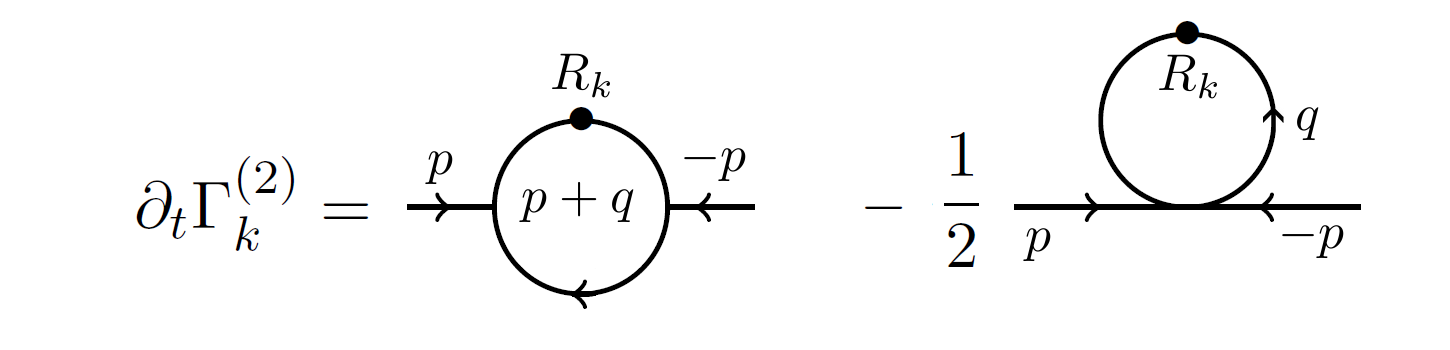
\includegraphics[scale=0.4]{Immagini/grafiloop.png}
\caption{A Feynman-like graph representation for $\Gamma^{(2)} = A - \frac{1}{2} B$}
\label{fig:loops}
\end{center}
\end{figure}

\subsection{Evolution of $Z_k(\rho)$}
Now, in order to perform the calculation of the exact evolution equation of $ Z_k(\rho)$, let's remember the expression of the second functional derivative of the effective average action:
\begin{displaymath}\label{G2}
\left.
\begin{array}{l}
 \frac{\delta^2 \Gamma_{k}}{\delta\phi_a(p)\delta\phi_b(-p)} =  \delta^{ab}U'_k(\rho) + \phi^a\phi^bU''_k(\rho)+ Z_k(\rho) p^2 \delta_{ab} + \rho Y_k(\rho) p^2\widehat{\phi}_a\widehat{\phi}_b  = \\ \\
 = \left[U'_k(\rho) +  Z_k(\rho)p^2\right](\delta_{ab} - \widehat{\phi}_a\widehat{\phi}_b) + \left[U'_k(\rho) + 2\rho U''_k(\rho) + \big(Z_k(\rho) + \rho Y_k(\rho)\big)p^2\right]\widehat{\phi}_a\widehat{\phi}_b\ = \\ \\ 
 \end{array}
\right.
\end{displaymath}
So, if we perform a derivative respect to $p^2$ (the exact meaning of which will be defined in the following) and take the 
longitudinal component of the previous expression, we obtain:
\begin{equation}\label{(42)}
 Z_k(\rho) = \left. \frac{\delta_{ab} - \widehat{\phi}_a\widehat{\phi}_b}{N-1} \frac{\partial}{\partial p^2} \frac{\delta^2 \Gamma_{k}}{\delta\phi_a(p)\delta\phi_b(-p)}\right|_{p = 0} 
\end{equation}
Deriving it with respect to $t = \ln\left(\frac{k}{\Lambda}\right)$ and using equation \eqref{G2} we obtain the following expression for $\dot{Z}_k(\rho)$:
$$\dot{Z}_k(\rho) = \left. \frac{\delta_{ab} - \widehat{\phi}_a\widehat{\phi}_b}{N-1} \frac{\partial}{\partial p^2}     \left(A - \frac{B}{2}\right)        \right|_{p = 0} \Def \dot{Z}^I_k(\rho) + \dot{Z}^{II}_k(\rho)$$
where I have defined $\dot{Z}^I_k(\rho)$ as the first graph contribution to the evolution of $Z_k(\rho)$ and $\dot{Z}^{II}_k(\rho)$ as the contribution due to the second graph. 

I will start from the evaluation of $\dot{Z}^{II}_k(\rho)$:
\begin{equation*}
 \dot{Z}^{II}_k(\rho) = -\frac{\delta_{ab} - \widehat{\phi}_a\widehat{\phi}_b}{2(N-1)} \frac{\partial}{\partial p^2}\left[\int \frac{d^Dq}{(2\pi)^D}G^{a_1a_3}(q)\Gamma^{(4)aba_3a_6}(p, -p, q, -q) G^{a_1a_3}(q)\dot{R}^{a_2a_1}_k(q)\right]_{p=0} = 
\end{equation*}
\begin{equation}\label{zetapunto2}
= -\frac{\delta^{ab} - \widehat{\phi}^a\widehat{\phi}^b}{2(N- 1)}\int \frac{d^Dq}{(2\pi)^D}\dot{R}_k(q)\left[(\delta^{a_3a_6} - \widehat{\phi}^{a_3}\widehat{\phi}^{a_6})G_{\perp}^2 + \widehat{\phi}^{a_3}\widehat{\phi}^{a_6}G_{\parallel}^2 \right]\left(\frac{\partial}{\partial p^2}\Gamma^{(4)}(p,-p,q,-q)\right)
\end{equation}

To go on with the evaluation it is now necessary to calculate the fourth functional derivative respect to the fields of the effective average action
\eqref{azioneefficace}. To simplify as much as possible the problem
we will use what is called the \emph{almost-constant fields approximation}. That consists in considering a large constant background field $\bar{\phi}$ and small 
space-dependent fluctuations around that:
\begin{equation}
 \phi^i(x) = \bar{\phi}^i + \delta \phi^i(x) 
\end{equation}
Concretely, that is equivalent in evaluating the functional derivatives of the effective average action 
(or the \emph{running proper vertices}) putting all the field's spacetime derivatives equal to zero at the end of the calculation.
That is done for every functional derivative of the effective average action up to order four in appendix A. 
It is a very long and tedious calculation, so here I will just state the result for $\Gamma^{(4)}$:
$$\Gamma^{(4)}(p, -p,q, -q) = (\delta^{ab}\delta^{a_3{a_6}} + \delta^{ad}\delta^{bc} + \delta^{ac}\delta^{bd})U_k''(\rho)+(2\rho)^2\widehat{\phi}^a\widehat{\phi}^b\widehat{\phi}^{a_3}\widehat{\phi}^{a_6} +$$
$$+2\rho(\delta^{ab}\widehat{\phi}^{a_3}\widehat{\phi}^{a_6} + \delta^{ad}\widehat{\phi}^b\widehat{\phi}^{a_3} + \delta^{ac}\widehat{\phi}^b\widehat{\phi}^{a_6} + \delta^{bc}\widehat{\phi}^a\widehat{\phi}^{a_6} + \delta^{bd}\widehat{\phi}^a\widehat{\phi}^{a_3} + \delta^{cd}\widehat{\phi}^a\widehat{\phi}^b)U_k'''(\rho) +$$
$$+Z_k'(\rho)\Big[p^2\delta^{ab}\delta^{cd} + 2 p\cdot q(\delta^{ad}\delta^{bc} - \delta^{ac}\delta^{bd}) + q^2\delta^{ab}\delta^{cd}\Big] + $$
$$+2\rho Z_k''(\rho)\Big[p^2\delta^{ab} \widehat{\phi}^{a_3}\widehat{\phi}^{a_6} + p\cdot q(\delta^{ad}\widehat{\phi}^b\widehat{\phi}^{a_3}  - \delta^{ac}\widehat{\phi}^b\widehat{\phi}^{a_6} +\delta^{bc}\widehat{\phi}^a\widehat{\phi}^{a_6} - \delta^{bd}\widehat{\phi}^a\widehat{\phi}^{a_3}) + q^2 \delta^{cd}\widehat{\phi}^a\widehat{\phi}^b \Big] +$$
$$+ \frac{Y_k(\rho)}{2}\Big[p^2(\delta^{ac}\delta^{bd} + \delta^{ac}\delta^{bd}) + q^2(\delta^{bc}\delta^{ad} + \delta^{ac}\delta^{bd}) + 2p\cdot q (\delta^{ac}\delta^{bd} - \delta^{bc}\delta^{ad})\Big] +$$
$$+2\rho^2Y''_k(\rho)(p^2 + q^2)\widehat{\phi}^a\widehat{\phi}^b\widehat{\phi}^{a_3}\widehat{\phi}^{a_6}+\rho Y'_k(\rho)\Big[p^2(\delta^{ac}\widehat{\phi}^b\widehat{\phi}^{a_6} + \delta^{bc}\widehat{\phi}^a\widehat{\phi}^{a_6} + \delta^{ad}\widehat{\phi}^b\widehat{\phi}^{a_3} + \delta^{bd}\widehat{\phi}^a\widehat{\phi}^{a_3} + \delta^{cd}\widehat{\phi}^a\widehat{\phi}^b) + $$
$$p\cdot q(\delta^{ac}\widehat{\phi}^b\widehat{\phi}^{a_6} + \delta^{bd}\widehat{\phi}^a\widehat{\phi}^{a_3} - \delta^{b{a_3}}\widehat{\phi}^a\widehat{\phi}^{a_6} - \delta^{a{a_6}}\widehat{\phi}^b\widehat{\phi}^{a_3}) + $$
$$ + q^2(\delta^{ad}\widehat{\phi}^b\widehat{\phi}^{a_3} +  \delta^{ab}\widehat{\phi}^{a_3}\widehat{\phi}^{a_6} + \delta^{ac}\widehat{\phi}^b\widehat{\phi}^{a_6} + \delta^{bc}\widehat{\phi}^a\widehat{\phi}^{a_6} + \delta^{bd}\widehat{\phi}^a\widehat{\phi}^{a_3})\Big] $$
The $p\cdot q$ terms do not contribute to $\dot{Z}^{II}_k(\rho)$ because of rotational invariance of the space of integration and because the other functions in the integral depends just on $q^2$:
\begin{equation}
 \int\frac{d^Dq}{(2\pi)^D} (p \cdot q)f(q^2) = 0
\end{equation}
Therefore we can ignore the irrelevant $p\cdot q$ terms and perform the $p^2$-derivative of $\Gamma^{(4)}$:
$$\frac{\partial}{\partial p^2}\Gamma^{(4)}(p,-p,q,-q) = Z'_k(\rho)\delta^{ab}\delta^{{a_3}{a_6}} + 2\rho Z''_k(\rho)\delta^{ab}\widehat{\phi}^{a_3}\widehat{\phi}^{a_6} + $$
$$ + \frac{Y_k(\rho)}{2}(\delta^{aa_6}\delta^{ba_3} + \delta^{aa_3}\delta^{ba_6}) + 2\rho^2Y''_k(\rho)\widehat{\phi}^{a}\widehat{\phi}^{b}\widehat{\phi}^{a_3}\widehat{\phi}^{a_6} + $$
\begin{equation}
+\rho Y'_k(\rho)(\delta^{aa_3}\widehat{\phi}^{b}\widehat{\phi}^{a_6} + \delta^{ba_3}\widehat{\phi}^{a}\widehat{\phi}^{a_6} + \delta^{aa_6}\widehat{\phi}^{b}\widehat{\phi}^{a_3} + \delta^{ba_6}\widehat{\phi}^{a}\widehat{\phi}^{a_3} + \delta^{a_3a_6}\widehat{\phi}^{a}\widehat{\phi}^{b})
\end{equation}
Substituting this in equation \eqref{zetapunto2} we obtain, after contracting the $O(N)$ indices:
\begin{equation}
 \dot{Z}_k^{II}(\rho) = -\frac{1}{2}\int\frac{d^Dq}{(2\pi)^D}\dot{R}(q)\left[((N-1)Z'_k(\rho) + Y_k(\rho))G^2_\perp(q) + (Z_k'(\rho) + 2\rho Z''_k(\rho))G^2_\parallel(q)\right]
\end{equation}
The evaluation of the other graph is quite similar. For the sake of brevity I will not rewrite the entire calculation,
but I will only give a sketch of the procedure. The starting point is obviously the expression of $\dot{Z}^{I}_k(\rho)$:
\begin{equation}
\dot{Z}^{I}_k(\rho) = \frac{\delta_{ab} - \widehat{\phi}_a\widehat{\phi}_b}{N-1} \frac{\partial}{\partial p^2}\left[\int \frac{d^Dq}{(2\pi)^D} {G}_k^{a_1a_3}(q) {\Gamma}^{(3)aa_3a_4}_{(p, q, -p-q)} {G}_k^{a_4a_5}(p + q){\Gamma}^{(3)ba_5a_6}_{(-p,-q,p+q)}{G}_k^{a_6a_2}(q)\dot{R}^{a_2a_1}_k(q)\right]_{p=0} =
\end{equation}
Making explicit all the terms in the integrand (the explicit expression of $\Gamma^{(3)}$ in the constant fields approximation and in momentum space can be found in the
Appendix A) and performing the $p^2$ derivative the final result can be derived after a long but not difficult calculation.
In performing the derivative respect to $p^2$ the following identities have been used:
\begin{enumerate}
\item $$ \int\frac{d^Dq}{(2\pi)^D} (p \cdot q)f(q^2) = 0$$
\item $$\int\frac{d^Dq}{(2\pi)^D} (p \cdot q)^2 f(q^2) = \frac{1}{D} \int\frac{d^Dq}{(2\pi)^D} p^2  q^2 f(q^2)$$
\end{enumerate}
and the following series expansion of the propagator:
$$G^{ij}([p+q]^2) = G^{ij}(p^2+2p\cdot q+q^2) = G^{ij}(q^2) + (p^2 + 2p\cdot q)G'^{ij}(q^2))+ 2(p\cdot q)^2G''^{ij}(q^2) + O(p^3)$$
Here $G^{ij}$ is considered as a function of $q^2$ and the primes denote derivatives with respect $q^2$. 
The finale result for $\dot{Z}^{II}_k(\rho)$ is:
\begin{equation}
\dot{Z}^{II}_k(\rho) = \frac{\rho}{D}\int \frac{d^Dq}{(2\pi)^D}\dot{R}_k(q)\Big\{2G^2_\perp(q)G_\parallel(q)(D+2)q^2Y^2_k(\rho)-8Z_k'(\rho)Y_k(\rho)G^2_\perp(q) G_\parallel(q) q^2+
\end{equation}
$$+ 4q^2(Z_k(\rho))^2G^2_\perp(q) G_\parallel(q) + 4DY_k(\rho)U''_k(\rho)G^2_\perp(q) G_\parallel(q) + Y_k^2(\rho)G^2_\perp(q) G'_\parallel(q) (D+8) q^4 - 8Y_k(\rho)Z_k'(\rho)G^2_\perp(q) G'_\parallel(q) q^4+$$
$$+2U''_k(\rho)Y_k(\rho)G^2_\perp(q) G'_\parallel(q) (D+8)q^2 - 16U''_k(\rho)G^2_\perp(q) G'_\parallel(q) Z'_k(\rho)q^2 + 2q^6Y^2_k(\rho)G^2_\perp(q) G_\parallel(q) + $$
$$+ 2Dq^2G^2_\perp(q) G'_\parallel(q) Y_k(\rho)U''_k(\rho) + 4q^4G^2_\perp(q) G''_\parallel(q) U''_k(\rho)Y_k(\rho) +4DG^2_\perp(q) G'_\parallel(q) (U''_k(\rho))^2 + $$
$$+4DG'_\perp(q) G^2_\parallel(q) (U''_k\rho))^2 + 8q^2G''_\perp(q) G^2_\parallel(q) (U''_k(\rho)^2) + 4q^2G_\perp(q) G^2_\parallel(q)(Z'_k(\rho)^2 + 8G^2_\parallel(q) Z'_k(\rho)(DG_\perp(q) +  $$
$$+ Y^2_k(\rho)G^2_\parallel(q)(DG'_\perp(q) + 2q^2G'_\perp(q))U''_k(\rho)) + 8q^2(U''_k(\rho))^2G^2_\perp(q) G''_\parallel(q) +4q^2Y_k(\rho)G^2_\perp(q) G''_\parallel(q) U''_k(\rho)+$$
$$ + 2q^2G''_\perp(q))q^4 + 4G^2_\parallel(q) Y_k(\rho)Z'_k(\rho)(DG_\perp(q) + 2q^2G'_\perp(q)) + 4G^2_\parallel(q) U''_k(\rho)Y_k(\rho)(DG'_\perp(q) + 2q^2G''_\perp(q))q^2$$

\subsection{Evolution of $Y_k(\rho)$}
Instead of deriving the evolution equation of $Y_k(\rho)$ we will calculate the evolution of an equivalent quantity, 
defined in the following way:
\begin{equation}
 \widetilde{Z}_k(\rho) = Z_k(\rho) + \rho Y_k(\rho)
\end{equation}
according to what is usually done in the literature. The evolution equation for $Y_k (\rho)$  can obviously be deduced from the one for $\widetilde{Z}_k(\rho)$ knowing the expression of $Z_k(\rho)$, 
derived in the previous section. From equation \eqref{G2} we obtain:
\begin{equation}\label{(43)}
 \widetilde{Z}_k(\rho) = \left. \widehat{\phi}_a\widehat{\phi}_b \frac{\partial}{\partial p^2} \frac{\delta^2 \Gamma_{k}}{\delta\phi_a(q)\delta\phi_b(-q)}\right|_{p = 0}
\end{equation}
The procedure is exactly the same just seen for $\dot{Z}_k(\rho)$, so I will only state the results:
\begin{equation}
 \dot{\widetilde{Z}}_k(\rho) = \dot{\widetilde{Z}}^{I}_k(\rho) + \dot{\widetilde{Z}}^{II}_k(\rho)
\end{equation}
Where I have separated the two graph contributions:
\small{
$$\dot{\widetilde{Z}}^{I}_k(\rho) = \frac{1}{D} \int\frac{d^Dq}{(2\pi)^D}\dot{R}_k(q) 2\rho \Big\{(N-1)G_\perp^2(q)\big[G_\perp\big(q^2Z'_k(\rho)(DY_k + Z'_k(\rho)) + DY_k(\rho)U''_k(\rho)\big) + $$ 
$$ + (q^2Z'_k(\rho) + U''_k(\rho))\big(2q^2G''_\perp(q)(q^2Z'_k(\rho)+ U''_k(\rho)) + G'_\perp(q^2)((4+D)q^2Z'_k(\rho) + DU''_k(\rho))\big]+$$
$$+ G_\parallel^2(q)\big[G_\parallel(q)(Y_k(\rho) + \rho Y'_k(\rho) + Z'_k(\rho))\Big(q^2\big(Z'_k(\rho) + (2D + 1)(Y'_k(\rho) + \rho Y'_k(\rho) + 2DZ'_k(\rho))\big) + 2D(3U''_k(\rho) + 2\rho U'''_k(\rho))\Big) + $$
$$ + \Big(q^2(Y_k(\rho) + \rho Y'_k(\rho) + 2Z'_k(\rho) + 3U''_k(\rho) + 2\rho U'''_k(\rho)\Big)\Big[G'_\parallel(q)\Big((D+4)q^2(\rho Y'_k(\rho) + Z'_k(\rho)) +D(3U''_k(\rho) + 2\rho U'''_k(\rho))\Big) + $$
$$ + 2q^2\big( \frac{Y_k(\rho)}{2}((4+D)G'_\parallel(q) + 2q^2G''_\parallel(q)) + G''_\parallel (q^2(\rho Y'_k(\rho) + Z'_k(\rho)) + 3U''_k(\rho) + 2\rho U'''_k(\rho))  \big) \Big]\Big\} $$}
and:
\small{
$$\dot{\widetilde{Z}}^{II}_k(\rho) = - \frac{1}{2} \int\frac{d^Dq}{(2\pi)^D}\dot{R}_k(q)\Big[\big(Z'_k(\rho) + \rho Y'_k(\rho)\big)(N-1)G^2_\perp(q) + \big(Z'_k(\rho) + 2\rho Z''_k(\rho) + Y_k(\rho) + 5\rho Y_k'\rho + 2\rho^2 Y''_k(\rho)\big)G^2_\parallel(q) \Big]$$}


\section{Dimensionless quantities}
A fixed point can be defined only in terms of dimensioless quantities, so I have defined the new dimensionless variables, following what is usually done in the literature. All the definitions are summarized in table \ref{tab:DIMENSIONLESS}.


\begin{table}
  \begin{center}
    \begin{small}
      \begin{tabular}{|c|c|c|}

\hline
 \textbf{Symbol}& \textbf{Definition} & \textbf{Description}  \\
\hline
$Z_k$ & $Z_k(\rho_0)$ & wavefunction renormalization at the minimum of the potential\\
\hline
$\rho_0$ & $U'_k(\rho_0) = 0$ & field strength at potential minimum\\
\hline
$\widetilde{\rho}$ & $Z_kk^{2-D}\rho$ & dimensionless field strength \\
\hline
$r(y)$ & $Z^{-1}_k q^{-2}R_k(q)$ & dimensionless regulator\\
\hline
$v_D$ & $[(2^{D + 1}\pi^{D/2}\Gamma(D/2)]^{-1}$ & $v_D$ factor\\
\hline
$y$ & $q^2/k^2$ & dimensionless momentum\\
\hline
$\eta_k$ & $-\dot{Z}_k/Z_k$ & anomalous dimension\\
\hline
$u_k(\widetilde{\rho})$ & $k^{-D}U_k(\widetilde{\rho})$ & renormalized potential\\
\hline
$z_k(\rho)$ & $Z_k(\rho)/Z_k$ & renormalized $Z_k(\rho)$\\
\hline
$\mathcal{Y}_k(\widetilde{\rho})$ & $Z_k^{-2}k^{D-2}Y_k(\rho)$ & renormalized $Y_k(\rho)$\\
\hline
      \end{tabular}
    \end{small}
  \end{center}
\caption{Table of the dimensionless variable used in this thesis, with their definitions and their physical descriptions.}
\label{tab:DIMENSIONLESS}

\end{table}


Now we can rewrite the flow equation in terms of the new variables. 
In the left hand side of all of the flow equations we have a derivative of the observable under examination with respect to $t$, calculated at fixed $\rho$. In order to obtain
an equivalent expression for that flow equation we need to express that in terms of a derivative calculated for a fixed value of $\widetilde{\rho}$.
We have:
\begin{equation*}
 \left. \frac{\partial}{\partial t} \right|_{\widetilde{\rho}} = \left. \frac{\partial}{\partial t} \right|_\rho + \left. \frac{\partial\rho}{\partial t} \right|_{\widetilde{\rho}}\left.\frac{\partial}{\partial\rho}\right|_t =
\end{equation*}
\begin{equation*}
\left.\left. \frac{\partial}{\partial t} \right|_\rho + \left.\left.\frac{\partial\ln{\widetilde{\rho}}}{\partial\ln{\rho}}\right|_t\left.\frac{\partial\ln(\rho)}{\partial t}\right|_{\widetilde{\rho}}\widetilde{\rho}\frac{\partial}{\partial\widetilde{\rho}}\right|_t =  \left. \frac{\partial}{\partial t} \right|_{\rho} + (D- 2 + \eta)\widetilde{\rho}\frac{\partial}{\partial\widetilde{\rho}}\right|_t
\end{equation*}
It will be useful, in the following, also the expression:
\begin{equation}
\frac{\dot{R}_k(q^2)}{Z_k q^2} =  \frac{1}{Z_k}\frac{\partial}{\partial t} \frac{R_k(q^2)}{q^2} = \frac{\partial}{\partial t} r_k(q^2) +\frac{\partial}{\partial t}(\ln Z_k)r(y) =  (\partial_t - \eta) r(y) =  -(2y\partial_y + \eta) r(y)
\end{equation}
The last thing to do is to find a renormalized expression for the two projection of the propagator, $G_\perp(q^2)$ and $G_\parallel(q^2)$.
In order to do this, we will calculated the renormalized expressions for each observable in the definition of those projection.
\begin{enumerate}
 \item $$U_k'(\rho) = \frac{\partial \widetilde{\rho}}{\partial \rho}\partial_{\widetilde{\rho}}[k^Du_k(\widetilde{\rho})] = Z_kk^2u_k'(\widetilde{\rho})$$
 \item $$Z_k(\rho)q^2 = Z_kk^2z_k(\widetilde{\rho})y$$
 \item $$R_k(q^2) = Z_kq^2r_k(q^2) = Z_kk^2r_k(y)y$$
 \item $$2\rho U_k''(\rho) = 2\frac{\widetilde{\rho}}{Z_k k^{2-D}}\left(\frac{\partial\widetilde{\rho}}{\partial{\rho}}\right)^2k^Du''_k(\widetilde{\rho}) = 2Z_kk^2\widetilde{\rho}u''_k(\widetilde{\rho})$$
 \item $$\rho Y_k(\rho)q^2 = \frac{\widetilde{\rho}}{Z_kk^{2-D}}q^2Z_k^2k^{2-D}\mathcal{Y}_k(\widetilde{\rho}) = Z_kk^2\widetilde{\rho}y\mathcal{Y}_k(\widetilde{\rho})$$
\end{enumerate}
So, we have obtained the following expression for the renormalized projections of the exact propagator:
\begin{equation}
 G_\perp(q^2) = \frac{g_\perp(y)}{Z_kk^2}
\end{equation}
\begin{equation}
 G_\parallel(q^2) = \frac{g_\parallel(y)}{Z_kk^2}
\end{equation}
where the dimensionless quantities $g_\perp$ and $g_\parallel$ are defined in the following way:
$$g_\perp(y) = \frac{1}{u_k'(\widetilde{\rho}) + [z_k(\widetilde{\rho}) + r_k(y)]y}$$
$$g_\parallel(y) = \frac{1}{u_k'(\widetilde{\rho}) + 2\widetilde{\rho}u_k''(\widetilde{\rho})+ [z_k(\widetilde{\rho}) + \widetilde{\rho}\mathcal{Y}_k(\widetilde{\rho})+ r_k(y)]y}$$

\subsection{The flow equation for the dimensionless potential}
In order to obtain the flow equation for the dimensionless potential $u_k(\widetilde{\rho})$, first of all we have to rewrite eq.\eqref{upunto} in terms of $\widetilde{\rho}$.
The result is:
\begin{equation}
\left.\frac{\partial}{\partial t} U_k(\widetilde{\rho})\right|_{\widetilde{\rho}} = (D - 2 + \eta)\widetilde{\rho}\frac{\partial U_k(\widetilde{\rho})}{\partial \widetilde{\rho}} + v_dk^{-2} \int_0^\infty (q^2)^{\frac{D}{2}}  \frac{\dot{R}_k(q^2)}{q^2} \left[(N-1)G_\perp(q^2)  + G_\parallel(q^2)\right] d(q^2)
\end{equation}
where I have already changed the integration variable to $q^2$. Now, remembering the definitions of $g_\perp$ and $g_\parallel$, I multiply and divide for $Z_k$ in the integral:
\begin{equation}
\left.\frac{\partial}{\partial t} U_k(\widetilde{\rho})\right|_{\widetilde{\rho}} = (D - 2 + \eta)\widetilde{\rho}\frac{\partial U_k(\widetilde{\rho})}{\partial \widetilde{\rho}} + v_d \int_0^\infty (q^2)^{\frac{D}{2}}  \frac{\dot{R}_k(q^2)}{Z_k (q^2)} \left[ (N-1)g_\perp(q^2)  + g_\parallel(q^2)\right] d(q^2)
\end{equation}
Now we can substitute the dimensionless potential $u_k(\widetilde{\rho}) = k^{-D}U_k(\widetilde{\rho})$. The left hand side becomes:
\begin{equation}
\left.\frac{\partial}{\partial t} U_k(\widetilde{\rho})\right|_{\widetilde{\rho}} = \left.\frac{\partial}{\partial t} [k_Du_k(\widetilde{\rho})]\right|_{\widetilde{\rho}} = k^D\dot{u}(\widetilde{\rho}) + D k^D u_k(\widetilde{\rho})
\end{equation}
So:
\begin{equation}
\dot{u}(\widetilde{\rho}) = -D  u_k(\widetilde{\rho}) +(D - 2 + \eta)\widetilde{\rho}\frac{\partial u_k(\widetilde{\rho})}{\partial \widetilde{\rho}} + v_d \int_0^\infty \frac{(q^2)^{\frac{D}{2}}}{k^D}  \frac{\dot{R}_k(q^2)}{Z_k q^2} \left[  (N-1)g_\perp   + g_\parallel \right] d(q^2) 
\end{equation}
By substituting the definition of $y $ we obtain:
\begin{equation}
\dot{u}(\widetilde{\rho}) = -D  u_k(\widetilde{\rho}) +(D - 2 + \eta)\widetilde{\rho}\frac{\partial u_k(\widetilde{\rho})}{\partial \widetilde{\rho}} + v_d \int_0^\infty y^{\frac{D}{2}}  (\partial_t - \eta) r_k(y) \left[ (N-1){g_\perp}  + g_\parallel \right] dy
\end{equation}
Where I have used the fact that the dimensionless regulator function is function of $y$.

In terms of the threshold function, which I have defined in Appendix C, the flow equation just derived is written in the following way:
\begin{equation}
 \dot{u}(\widetilde{\rho}) = -D  u_k(\widetilde{\rho}) +(D - 2 + \eta)\widetilde{\rho}u'_k(\widetilde{\rho}) + v_d \big((N - 1)L^D_{1,0} + L^D_{0,1} \big)
\end{equation}



\subsection{The flow equation for $z_k(\widetilde{\rho})$}
We can now find the flow equation for the regularized wavefunction renormalization in terms of adimensional quantities.
Obviously, the derivative of $Z_k(\widetilde{\rho})$ becomes:
\begin{equation*}
 \dot{Z}_k(\widetilde{\rho}) = \dot{Z}_k(\rho) + (D-2+\eta)\widetilde{\rho}\frac{\partial}{\partial \widetilde{\rho}}Z_k(\widetilde{\rho})
\end{equation*}
and, substituting the definition of $z_k(\widetilde{\rho})$ and remembering the definitions of the two graphs contributes:
\begin{equation}
\dot{z}_k(\widetilde{\rho}) =  (D-2+\eta)\widetilde{\rho}\frac{\partial}{\partial \widetilde{\rho}} z_k(\widetilde{\rho}) + \eta z_k(\widetilde{\rho}) + \frac{\dot{Z}^I_k(\widetilde{\rho})}{Z_k} + \frac{\dot{Z}^{II}_k(\widetilde{\rho})}{Z_k} 
\end{equation}
Now we have to deduce the renormalized expressions for the two graph. Let's start from $\dot{Z}^{II}_k(\widetilde{\rho})/Z_k$:
\begin{equation*}
 \dot{z}^{II}_k(\widetilde{\rho}) = \frac{\dot{Z}^{II}_k(\widetilde{\rho})}{Z_k} =  -\frac{1}{2Z_k}\int\frac{d^Dq}{(2\pi)^D}\dot{R}(q)\left[((N-1)Z'_k(\rho) + Y_k(\rho))G^2_\perp(q) + (Z_k'(\rho) + 2\rho Z''_k(\rho))G^2_\parallel(q)\right]=
\end{equation*}
\begin{equation*}
=  -v_D\int_0^\infty dx x^{\frac{D}{2}}\frac{\dot{R}(x)}{Z_kx}\left[\left((N-1)\frac{Z_k^2}{k^{D-2}}z'_k(\widetilde{\rho}) + \frac{Z_k^2}{k^{D-2}}\mathcal{Y}_k(\widetilde{\rho})\right)\frac{g^2_\perp(x)}{Z^2_kk^4} + \left(\frac{Z_k^2z'_k(\widetilde{\rho})}{k^{D-2}} + \frac{2\widetilde{\rho} z''_k(\widetilde{\rho})Z_k^2}{k^{D-2}}\right)\frac{g^2_\parallel(x)}{Z^2_kk^4}\right]=
\end{equation*}
\begin{equation}
=  v_D\int_0^\infty dy y^{\frac{D}{2}}  (2y\partial_y + \eta) r_k(y)\left[\left((N-1)z'_k(\widetilde{\rho}) + \mathcal{Y}_k(\widetilde{\rho})\right)g^2_\perp(y) + \left(z'_k(\widetilde{\rho}) + 2\widetilde{\rho} z''_k(\widetilde{\rho})\right)g^2_\parallel(y)\right]
\end{equation}
In a quite similar way, we find the renormalized expression of the other graph:
\begin{equation} 
\dot{z}^{I}_k(\widetilde{\rho}) = \frac{\dot{Z}^{I}_k(\widetilde{\rho})}{Z_k} = 
\end{equation}
$$-\frac{2 \widetilde{\rho}v_D}{D}\int_0^\infty dy(2y\partial_y + \eta_k)r_k(y)\Big\{2g^2_\perp(y)g_\parallel(y)(D+2)y\mathcal{Y}^2_k(\widetilde{\rho})-8z_k'(\widetilde{\rho})\mathcal{Y}_k(\widetilde{\rho})g^2_\perp(y) g_\parallel(y) y+$$
$$+ 4y(z_k(\widetilde{\rho}))^2g^2_\perp(y) g_\parallel(y) + 4D\mathcal{Y}_k(\widetilde{\rho})u''_k(\widetilde{\rho})g^2_\perp(y) g_\parallel(y) + \mathcal{Y}_k^2(\widetilde{\rho})g^2_\perp(y) g'_\parallel(y) (D+8) y^4 - 8\mathcal{Y}_k(\widetilde{\rho})z_k'(\widetilde{\rho})g^2_\perp(y) g'_\parallel(y) y^2+$$
$$+2u''_k(\widetilde{\rho})\mathcal{Y}_k(\widetilde{\rho})g^2_\perp(y) g'_\parallel(y) (D+8)y - 16u''_k(\widetilde{\rho})g^2_\perp(y) g'_\parallel(y) z'_k(\widetilde{\rho})y + 2y^3\mathcal{Y}^2_k(\widetilde{\rho})g^2_\perp(y) g_\parallel(y) + $$
$$+ 2Dyg^2_\perp(y) g'_\parallel(y) \mathcal{Y}_k(\widetilde{\rho})u''_k(\widetilde{\rho}) + 4y^2g^2_\perp(y) g''_\parallel(y) u''_k(\widetilde{\rho})\mathcal{Y}_k(\widetilde{\rho}) +4Dg^2_\perp(y) g'_\parallel(y) (u''_k(\widetilde{\rho}))^2 + $$
$$+4Dg'_\perp(y) g^2_\parallel(y) (u''_k\widetilde{\rho}))^2 + 8yg''_\perp(y) g^2_\parallel(y) (u''_k(\widetilde{\rho})^2) + 4yg_\perp(y) g^2_\parallel(y)(z'_k(\widetilde{\rho})^2 + 8g^2_\parallel(y) z'_k(\widetilde{\rho})(Dg_\perp(y) +  $$
$$+ \mathcal{Y}^2_k(\widetilde{\rho})g^2_\parallel(y)(Dg'_\perp(y) + 2yg'_\perp(y))u''_k(\widetilde{\rho})) + 8y(u''_k(\widetilde{\rho}))^2g^2_\perp(y) g''_\parallel(y) +4y\mathcal{Y}_k(\widetilde{\rho})g^2_\perp(y) g''_\parallel(y) u''_k(\widetilde{\rho})+$$
$$ + 2yg''_\perp(y))y^2 + 4g^2_\parallel(y) \mathcal{Y}_k(\widetilde{\rho})z'_k(\widetilde{\rho})(Dg_\perp(y) + 2yg'_\perp(y)) + 4g^2_\parallel(y) u''_k(\widetilde{\rho})\mathcal{Y}_k(\widetilde{\rho})(Dg'_\perp(y) + 2yg''_\perp(y))y\Big\}$$
In terms of the threshold functions the equation for $\dot{{z}}^{I}_k(\widetilde{\rho})$ and  $\dot{{z}}^{II}_k(\widetilde{\rho})$ are:
$$\dot{z}^{I}_k(\widetilde{\rho}) =  4v_D \widetilde \rho u_k''(\widetilde \rho) Q^{D, 0}_{2, 1} + 4 v_D \mathcal{Y}_k u_k''(\widetilde \rho) Q^{D,1}_{2,1} + v_D \widetilde \rho \mathcal{Y}^2_k (\widetilde \rho)Q^{D,2}_{2,1}- 8 v_D \widetilde \rho z'_k(\widetilde \rho)u_k''(\widetilde \rho)L^D_{1,1}-$$
$$-\frac{4v_D}{D}\big(z_k'(\widetilde \rho)\big)^2\widetilde \rho L^{D+2}_{1,1} - 4v_D \widetilde \rho z_k'(\widetilde \rho) \mathcal{Y}_k(\widetilde \rho)L^{D+2}_{1,1} + \frac{16v_D}{D}\widetilde \rho z_k'(\widetilde \rho) u''_k(\widetilde \rho)N^D_{2,1} + \frac{8v_D}{D} \widetilde \rho z'_k(\widetilde \rho) \mathcal{Y}_k(\widetilde \rho)N^{D+2}_{2,1}$$

$$\dot{z}^{II}_k(\widetilde{\rho}) = - v_D\big[((N-1)z'_k(\widetilde{\rho}) + \mathcal{Y}_k(\widetilde{\rho}\big]L^D_{1,0} - v_D\big[z'_k(\widetilde{\rho}) + 2\widetilde{\rho} z''_k(\widetilde{\rho}\big]L^D_{0,1}$$
\subsection{The flow equation for $\widetilde{z}_k(\widetilde{\rho})$}
The procedure is very similar to what we've just seen for $\dot{z}_k(\widetilde{\rho})$ so here I will omit, for the sake of brevity, 
the details of the calculation, exposing only the final results. For the first graph we have:
$$\dot{\widetilde{z}}_k^{I}(\widetilde{\rho}) \equiv \frac{\dot{\widetilde{Z}}^{I}_k(\rho)}{Z_k} = - \frac{4\widetilde{\rho}v_D}{D} \int_0^\infty y(2y\partial_y + \eta_k)r_k(y) \Big\{(N-1)g_\perp^2(y)\big[g_\perp\big(yz'_k(\widetilde{\rho})(D\mathcal{Y}_k + z'_k(\widetilde{\rho})) + D\mathcal{Y}_k(\widetilde{\rho})u''_k(\widetilde{\rho})\big) + $$ 
$$ + (yz'_k(\widetilde{\rho}) + u''_k(\widetilde{\rho}))\big(2yg''_\perp(y)(yz'_k(\widetilde{\rho})+ u''_k(\widetilde{\rho})) + g'_\perp(y)((4+D)yz'_k(\widetilde{\rho}) + Du''_k(\widetilde{\rho}))\big]+$$
$$+ g_\parallel^2(y)\big[g_\parallel(y)(\mathcal{Y}_k(\widetilde{\rho}) + \widetilde{\rho} \mathcal{Y}'_k(\widetilde{\rho}) + z'_k(\widetilde{\rho}))\Big(y\big(z'_k(\widetilde{\rho}) + (2D + 1)(\mathcal{Y}'_k(\widetilde{\rho}) + \widetilde{\rho} \mathcal{Y}'_k(\widetilde{\rho}) + 2Dz'_k(\widetilde{\rho}))\big) + 2D(3u''_k(\widetilde{\rho}) + 2\widetilde{\rho} u'''_k(\widetilde{\rho}))\Big) + $$
$$ + \Big(y(\mathcal{Y}_k(\widetilde{\rho}) + \widetilde{\rho} \mathcal{Y}'_k(\widetilde{\rho}) + 2z'_k(\widetilde{\rho}) + 3u''_k(\widetilde{\rho}) + 2\widetilde{\rho} u'''_k(\widetilde{\rho})\Big)\Big[g'_\parallel(y)\Big((D+4)y(\widetilde{\rho} \mathcal{Y}'_k(\widetilde{\rho}) + z'_k(\widetilde{\rho})) +D(3u''_k(\widetilde{\rho}) + 2\widetilde{\rho} u'''_k(\widetilde{\rho}))\Big) + $$
$$ + 2y\big( \frac{\mathcal{Y}_k(\widetilde{\rho})}{2}((4+D)g'_\parallel(y) + 2yg''_\parallel(y)) + g''_\parallel (y(\widetilde{\rho} \mathcal{Y}'_k(\widetilde{\rho}) + z'_k(\widetilde{\rho})) + 3u''_k(\widetilde{\rho}) + 2\widetilde{\rho} u'''_k(\widetilde{\rho}))  \big) \Big]\Big\} $$
while, for the other one:
\begin{equation}
 \dot{\widetilde{z}}_k^{II}(\widetilde{\rho}) \equiv \frac{\dot{\widetilde{Z}}^{II}_k(\rho)}{Z_k} =
\end{equation}
$$=  \int_0^\infty dy (2y\partial_y + \eta_k)r_k(y)\Big[\big(z'_k(\widetilde{\rho}) + \widetilde{\rho} \mathcal{Y}'_k(\widetilde{\rho})\big)(N-1)g^2_\perp(y) + \big(z'_k(\widetilde{\rho}) + 2\widetilde{\rho} z''_k(\widetilde{\rho}) + \mathcal{Y}_k(\widetilde{\rho}) + 5\widetilde{\rho} \mathcal{Y}_k' + 2\widetilde{\rho}^2 \mathcal{Y}''_k(\widetilde{\rho})\big)g^2_\parallel(y) \Big]$$
In terms of the threshold functions:
\begin{equation}
\dot{\widetilde{z}}_k^{I}(\widetilde{\rho})= v_D\Big[(N-1)(u_k''(\widetilde \rho))^2\widetilde \rho Q^{D,0}_{3,0} + 4(N-1)\widetilde \rho z'_k(\widetilde \rho)u''_k(\widetilde \rho) Q^{D,1}_{3,0}+
\end{equation}
$$+2(N-1)\widetilde \rho(z'_k(\widetilde \rho))^2 Q^{D,2}_{3,0} + 2\widetilde \rho (3u''_k(\widetilde \rho))+ 2 u_k'''(\widetilde \rho)\widetilde \rho)^2\widetilde Q^{D,0}_{3,0}+$$
$$+4v_D(z'_k(\widetilde \rho) + \mathcal{Y}_k(\widetilde \rho) + \widetilde \rho\mathcal{Y}'_k(\widetilde \rho)) (3u_k''(\widetilde{\rho}) + 2u'''_k(\widetilde{\rho})) \widetilde Q^{D,1}_{3,0}+$$
$$+2v_D(z'_k(\widetilde \rho) + \mathcal{Y}_k(\widetilde \rho) + \widetilde \rho\mathcal{Y}'_k(\widetilde \rho))^2\widetilde Q^{D,2}_{3,0}+\frac{8(N-1)}{D}\widetilde \rho z'_k(\widetilde \rho)u''_k(\widetilde \rho)N^D_{3,0} + $$
$$+\frac{8(N-1)}{D}\widetilde \rho z^2_k(\widetilde \rho)N^{D+2}_{3,0} + \frac{8}{D}(z_k'(\widetilde \rho) + \mathcal{Y}_k(\widetilde \rho) + \widetilde \rho \mathcal{Y}_k(\widetilde \rho))(3 u''_k(\widetilde \rho) + 2 \widetilde \rho u'''_k(\widetilde \rho))\widetilde \rho \widetilde N^D_{3,0} + $$
$$-\frac{8\widetilde \rho}{D}(z'_k(\widetilde \rho) + \mathcal{Y}_k(\widetilde \rho) + \widetilde \rho \mathcal{Y}'_k(\widetilde \rho))^2\widetilde N^{D+2}_{3,0} - 2(N-1) \mathcal{Y}_k(\widetilde \rho) u''_k(\widetilde \rho)  \widetilde \rho L^D_{2,0} -$$
$$-v_D (N-1) \left(z_k'(\widetilde \rho)\mathcal{Y}_k(\widetilde \rho) + \frac{1}{D}\big(z_k'(\widetilde \rho)\big)^2\right)\widetilde \rho L^{D+2}_{2,0}-4\widetilde \rho (z'_k(\widetilde \rho) + \mathcal{Y}_k(\widetilde \rho) + \widetilde \rho \mathcal{Y}'_k(\widetilde \rho))(3 u''_k(\widetilde \rho) + 2 \widetilde \rho u'''_k(\widetilde \rho)) L^D_{0,2} -$$
$$-2v_D\left(2 + \frac{1}{D}\right)\widetilde \rho (z'_k(\widetilde \rho) + \mathcal{Y}_k(\widetilde \rho) + \widetilde \rho \mathcal{Y}'_k(\widetilde \rho))^2L^{D+2}_{0,2} $$
\begin{equation}
 \dot{\widetilde{z}}_k^{II}(\widetilde{\rho}) = v_D\Big[\big(z'_k(\widetilde{\rho}) + \widetilde{\rho} \mathcal{Y}'_k(\widetilde{\rho})\big)(N-1)L^D_{1,0} + \big(z'_k(\widetilde{\rho}) + 2\widetilde{\rho} z''_k(\widetilde{\rho}) + \mathcal{Y}_k(\widetilde{\rho}) + 5\widetilde{\rho} \mathcal{Y}_k' + 2\widetilde{\rho}^2 \mathcal{Y}''_k(\widetilde{\rho})\big)L^D_{0,1} \Big]
\end{equation}




\section{Large N limit}
We are interested now in studying the large N limit, when only transverse (or Goldstone) modes are involved in the dynamic 
of the system. In this limit, as can be easily checked (see, for example, \cite{morristurner}), the flow equation for $Y_k(\rho)$ is decoupled from the other two 
(or, equivalently, $\lim_{N\to \infty} \dot{{\widetilde{Z}}}_k(\rho) = \dot{Z}_k(\rho) $) and the problem simplify considerably.

Now I will derive the large N limits of the two flow equations for the dimensionless effective potential $u_k(\rho)$ and the renormalized wavefunction
renormalization $z_k(\rho)$. Then, these two will be object of a numerical evaluation, which will be started in the following chapter of this thesis.

\subsection{The effective potential evolution in the $N \to\infty$ limit}
In the large $N$ limit, we can keep only the terms of order $N$ in the flow equations. In the case of $\dot{u}_k$ that means:
\begin{equation}
\dot{u}(\widetilde{\rho}) = -D  u_k(\widetilde{\rho}) +(D - 2 + \eta)\widetilde{\rho}\frac{\partial u_k(\widetilde{\rho})}{\partial \widetilde{\rho}} - v_D \int_0^\infty y^{\frac{D}{2}}  (2y\partial_y + \eta_k) r_k(y) (N-1){g_\perp(y)} dy
\end{equation}
In order to perform the limit we need to rescale $u_k(\widetilde\rho)$ and $\rho$:
$$u \to \frac{u}{N} \ \ \ \ \ \ \ \ \ \  \ \ \ \ \ \  \ \ \ \ \ \ \  \ \ \ \ \ \   \widetilde{\rho} \to \frac{\widetilde{\rho}}{N} $$
And so we obtain the following expression:
\begin{equation}\label{upuntolargeN}
\dot{u}_k(\widetilde{\rho}) = -D  u_k(\widetilde{\rho}) +(D - 2 + \eta)\widetilde{\rho}\frac{\partial u_k(\widetilde{\rho})}{\partial \widetilde{\rho}} - v_D \int_0^\infty  \frac{y^{\frac{D}{2}} (2y\partial_y + \eta_k) r_k(y)}{y[z_k(\widetilde{\rho}) + r_k(y)] + u_k'(\widetilde{\rho})} dy 
\end{equation}


\subsection{The flow equation for $w_k(\widetilde{\rho}) \Def u'_k(\widetilde{\rho})$ in the large $N$ limit}
The study of the system in the large $N$ limit can be afford more easily considering, instead of the effective potential $u_k(\widetilde{\rho})$, its derivative $u'_k(\widetilde{\rho})$. Defining $w_k(\widetilde{\rho}) := u'_k(\widetilde{\rho})$ and deriving eq.\eqref{upuntolargeN} with respect to $\widetilde{\rho}$ one obtains:
\begin{equation}\label{wpuntolargeN}
 \dot{w}_k(\widetilde{\rho}) = (\eta_k -2 )w_k(\widetilde{\rho}) + (D-2 +\eta_k)\widetilde{\rho}\frac{\partial w_k(\widetilde{\rho})}{\partial \widetilde{\rho}} + v_D\int_0^\infty dy \frac{y^{\frac{D}{2}}  (2y\partial_y + \eta) r_k(y)(z'_k(\widetilde{\rho})y + w'_k(\widetilde{\rho}))}{\big([z_k(\widetilde{\rho}) + r_k(y)]y + w_k(\widetilde{\rho})\big)^2}
\end{equation}
For the sake of completeness, I will state the latter expression also in terms of the threshold function:
\begin{equation}
 \dot{w}_k(\widetilde{\rho}) = (\eta_k -2 )w_k(\widetilde{\rho}) + (D-2 +\eta_k)\widetilde{\rho}w'_k(\widetilde{\rho}) + v_Dw'_k(\widetilde{\rho})L^D_{1,0} + z'_kL^{D+1}_{1,0}
\end{equation}

\subsection{$z_k(\widetilde{\rho})$ flow equation in the $N \to\infty$ limit}
In the $N \to \infty$ limit, the only non-vanishing term in the exact evolution equation for the renormalized
wavefunction renormalization $z_k(\widetilde{\rho})$ is:
\begin{equation}
\dot{z}_k(\widetilde{\rho}) =\eta z_k(\widetilde{\rho}) + (D-2+\eta)\widetilde{\rho}\frac{\partial}{\partial \widetilde{\rho}} z_k(\widetilde{\rho}) + v_D\int_0^\infty dy y^{\frac{D}{2}}  (2y\partial_y + \eta_k) r_k(x)\left((N-1)z'_k(\widetilde{\rho})\right)g^2_\perp(y) 
\end{equation}
I will go on in analogy to what I've done for the effective potential equation, to perform the $N \to \infty$ limit, I need to rescale $u$ and $\widetilde{\rho}$:
$$u \to \frac{u}{N} \ \ \ \ \ \ \ \ \ \  \ \ \ \ \ \  \ \ \ \ \ \ \  \ \ \ \ \ \   \widetilde{\rho} \to \frac{\widetilde{\rho}}{N} $$
The result is:
\begin{equation}\label{zpuntolargeN}
\dot{z}_k(\widetilde{\rho}) =\eta z_k(\widetilde{\rho}) + (D-2+\eta)\widetilde{\rho}\frac{\partial}{\partial \widetilde{\rho}} z_k(\widetilde{\rho})  + v_D\int_0^\infty dy \frac{y^{\frac{D}{2}}  (2y\partial_y + \eta_k) r_k(y)z'_k(\widetilde{\rho})}{\big([z_k(\widetilde{\rho}) + r_k(y)]y + w_k(\widetilde{\rho})\big)^2}
\end{equation}
